\documentclass[12pt] {article}
\usepackage{times}
\usepackage[margin=1in,bottom=1in,top=1in]{geometry}

\usepackage{hhline}
\usepackage{subfig}
\usepackage[inline,shortlabels]{enumitem}%enumerate with letters
\usepackage[square,numbers]{natbib}
\usepackage{graphicx}
\bibliographystyle{unsrtnat}
\begin{document}

\title{Assignment One -  EEC254}
\author{Ahmed H. Mahmoud}
\date{January 23th, 2018}
\maketitle

%============Table========
%\begin{figure}[tbh]
% \centering    
%\begin{tabular}{ |p{4cm}|| p{2cm}|p{2cm}|p{2cm}|p{2cm}|}
% \hline
% & Processor 1 &  Processor 2  & Processor 3 & Processor 4\\ \hhline{|=|=|=|=|=|}
% \hline
% Performance          &$1.08$        &$1.425$       &\textbf{1.52}  &   \\
% \hline
%\end{tabular} 
%\caption{Metric table for the four processors}
%   \label{tab:metric}
%\end{figure} 
%============Figure========
%\begin{figure}[!tbh]
%\centering        
%   \subfloat {\includegraphics[width=0.65\textwidth]{fig2_4.png}}
%   \caption{ }
%   \label{fig:fig}
%\end{figure}



\paragraph{Problem 2.10} 
\begin{enumerate}[(a)]
\item The set $C = \left\lbrace x\in \mathcal{R}^n | x^{T}Ax + b^{T}x + c \leq 0 \right\rbrace$ is the solution of the function $f(x) = x^{T}Ax + b^{T}x + c$. Thus, proving that $f(x)$ directly implies that $C$ is also convex. 

To prove that $f(x)$ is convex, we need to prove the following $f(\mu x + (1-\mu)y) \leq \mu f(x) + (1-\mu)f(y), \forall \mu \in \left[0,1\right]$. Plugging in the definition of $f(x)$, we obtain the following 
$$
(\mu x + (1-\mu)y)^{T}A(\mu x + (1-\mu)y) + b^{T}(\mu x + (1-\mu)y) + c \leq  
$$
$$
\qquad \qquad \qquad \qquad \qquad \qquad \qquad \mu x^{T}Ax + \mu b^{T}x + \mu c + (1-\mu) y^{T}A y + (1-\mu) b^{T}y + (1-\mu) c 
$$
or 
$$
\mu^{2}x^{T}A x + (1-\mu)^{2}y^{T}A y + \mu(1-\mu)x^{T}A y + \mu(1-\mu)y^{T}A x + \mu b^{T} x + (1- \mu) b^{T} y + c \leq
$$
$$
\qquad \qquad \qquad \qquad \qquad \qquad \qquad \mu x^{T}A x + \mu  b^{T} x + \mu c + (1-\mu) y^{T}A y + (1-\mu) b^{T} y + (1-\mu) c
$$
The formula can be simplified to 
$$
\mu (1-\mu) x^{T} A x + \mu (1-\mu) y^{T} A y - \mu (1-\mu) x^{T}A y - \mu(1-\mu)y^{T}A x \geq 0
$$
$$
x^{T}Ax + y^{T}Ay - x^{T}Ay - y^{T}A x \geq 0
$$
$$
(x-y)^{T}A(x-y) \geq 0
$$
The final inequality is only possible iff $A$ is positive semidefinite i.e., $A \succeq 0$. The converse of this does not necessarily hold. 

\item 




\end{enumerate}

\paragraph{Problem 2.12} 
\begin{enumerate}[(a)]
\item A \emph{slab} can be expressed as half-spaces intersecting; the first set of half-spaces is of the form $\left\lbrace x \in \mathcal{R} | \alpha \leq a^{T} x \right\rbrace$ and the second set is $\left\lbrace x \in \mathcal{R} |  \leq a^{T} x \leq \beta \right\rbrace$. Since hyper-planes are both convex sets and intersection of two convex sets is a convex set, then a \emph{slab} is a convex set.

\item Geometrically, one can connect any two points inside a rectangle (or on its boundary) and the resulting line segment will be inside the rectangle (or on its boundary). Thus, a rectangle is a convex set. Additionally, a rectangle can be defined by intersection of half-spaces and thus it is convex.

\item Similar to slab, a \emph{wedge} is defined as intersection of half-spaces and thus it is convex. 

\item Geometrically, the set of points closer to a given points is also called \emph{Voronoi} diagram which can be easily constructed by intersection of half-spaces which makes it a convex set. 

\item If the given sets ($S, T$) are non-convex, it is likely that the set of point closer to on set than the other won't be convex; can not be constructed as a set of intersecting half-spaces. An example is shown in Figure \ref{fig:voro} (adapted from \citep{HELD2009327}) where the objects here is the thick solid curves and the set of points closer to one curve than the other is the generalized Voronoi diagram. At least one Voronoi cell can be identified as non convex (shown in a green circle). 
\begin{figure}[!tbh]
\centering        
   \subfloat {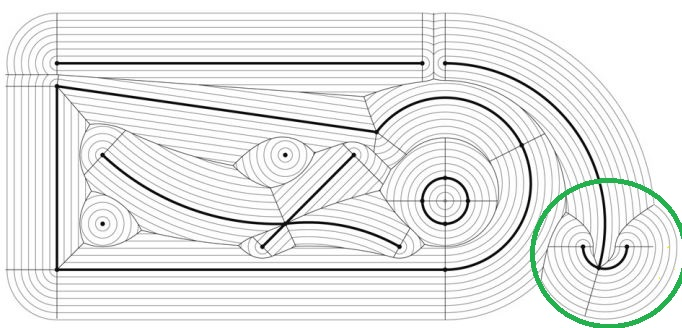
\includegraphics[width=0.65\textwidth]{fig/voro_curves.JPG}}
   \caption{Voronoi diagram (depicted by thin solid curves) and family of offset curves (grey) for a sample input (thick solid curves and isolated points). A non-convex cell is encircled in green. The figure is adapted from \citep{HELD2009327}.}
   \label{fig:voro}
\end{figure}

\item This set is convex. 

\item For the set $\left\lbrace x | ||x-a||_2 \leq \theta ||x-b||_2 \right\rbrace$, we manipulate its definition by taking the square of both side of the inequality; $\left\lbrace x | ||x-a||^{2}_{2} \leq \theta^{2} ||x-b||^{2}_{2} \right\rbrace$. The definition can further be expanded as follows 
$$\left\lbrace x |  (x-a)^{T}(x-a) \leq \theta^{2}(x-b)^{T}(x-b)\right\rbrace$$
$$=\left\lbrace x |  (x^{T}-a^{T})(x-a) \leq \theta^{2}(x^{T}-b^{T})(x-b)\right\rbrace$$
$$=\left\lbrace x |   x^{T}x + a^{T}a- 2a^{T}x \leq \theta^{2}(x^{T}x+b^{T}b-2b^{T}x) \right\rbrace$$
$$=\left\lbrace x |  (1-\theta^{2})x^{T}x - 2(a-\theta^{2}b)^{T}x \leq  \theta^{2}||b||^{2}_{2} - ||a||^{2}_{2} \right\rbrace$$
$$=\left\lbrace x |  x^{T}x - \frac{2(a-\theta^2b)^{T}}{1-\theta^2}x \leq  \frac{\theta^{2}||b||^{2}_{2} - ||a||^{2}_{2}}{1-\theta^2} \right\rbrace$$
which can finally be manipulated to make it looks like the definition of Euclidean ball centered at $x_{c}$ and of radius $r$ i.e., ${x |(x-x_{c})^{T}(x-x_{c})\leq r^{2}}$. Let $x_{c} = \frac{(a-\theta^2b)^{T}}{1-\theta^2}$

$$\left\lbrace x  |  x^{T}x - 2x_{c}x + ||x_{c}||^{2}_{2}  \leq  \frac{\theta^{2}||b||^{2}_{2} - ||a||^{2}_{2}}{1-\theta^2} + ||x_{c}||^{2}_{2} \right\rbrace$$
$$=\left\lbrace x |  (x-x_{c})^{T}(x-x_{c})  \leq  \frac{\theta^{2}||b||^{2}_{2} - ||a||^{2}_{2}}{1-\theta^2} + ||x_{c}||^{2}_{2} \right\rbrace$$
which is a ball centered at $x_{c}$ with radius equal to the square root of the right hand side of the inequality (which is constant). Thus, this set is convex. 
\end{enumerate}

\paragraph{Problem 2.16} 
Intuitively, since the partial sums is sums over two convex sets, then the result must be a convex set. More rigorously, we can apply the definition of the convex set on $S$ on any two points in $S$. The result will be summation of two convex combination one lies in $S_{1}$ and the other in $S_{2}$. Due to the convexity of $S_{1}$ and $S_{2}$, the convexity of the partial sum will follow. 

\paragraph{Problem 2.31}
\begin{enumerate}[(a)]
\item The definition of dual cone for the cone $K$ is $K^{*} = \left\lbrace y | x^{T}y\geq 0, \forall x \in K \right\rbrace$. The definition is a set of linear inequalities which can be represented by a set of intersecting half-spaces which is known to result into a convex set. 

\item If we have $y \in K^{*}_{2}$, then the definition of dual cone is applicable on it such that $x^{T}y\leq 0, \forall x \in K_{2}$ as shown in Figure \ref{fig:v}. Since $K_{1}$ already lives inside $K_{2}$, then we can restrict $x$  to be inside $K_{1}$. This will alter the definition to be $x^{T}y\leq 0, \forall x \in K_{1}$ which is the definition of dual cone of $K_{1}$. 

\item Since $K^{*}$ is the intersection of half-spaces, then it must be closed. 

\item \textit{(I was only able to reach a weak proof for this problem).} For the dual cone of $K$ that is defined as $K^{*} = \left\lbrace y | x^{T}y \geq 0, \forall x \in K \right\rbrace$, we can pick a point $y_{\circ} \in K^{*} $ such that there exists $x \in \mathbf{cl}\ K $ and it gives $y_{\circ}^{T}x=0$. That implies that $y_{\circ}$ must be on the boundary of $K^{*}$. Thus, in order to have $y_{\circ}$ such that $y_{\circ} \in \mathbf{int}\ K^{*}$, $y_{\circ}$ should satisfies that $y_{\circ}^{T}x < 0$ for some $x \in \mathbf{cl}\ K$. 

\item If $K^{*}$ is pointed, it means that there is no line in $K^{*}$ which implies that there no $y$ such that $y \in K^{*}$ and $-y \in K^{*}$. Given the definition of the dual cone $K^{*} = \left\lbrace y | x^{T}y\geq 0, \forall x \in K \right\rbrace$, in order to have a line in $K^{*}$, it means that $y^{T}x \leq 0$ and $-y^{T}x \leq 0$ which is only possible if $y^{T}x=0, \forall x \in K$. Recall that $y^{T}x=0$ is an equation of a single plane which implies that $K$ does not have an interior. Thus, if $K$ has nonempty interior then $K^{*}$ can not have a line i.e., is pointed. 

\item 

\item From (e) we have proven that if $K$ has nonempty interior then $K^{*}$ is pointed. We can apply the same logic between $K^{*}$ and $K^{**}$. We get then if $K^{*}$ has nonempty interior then $K^{**}$ is pointed. From (f), we have shown that $K^{**}$ is the closure of $K$. From that we end up that if $K^{*}$ has nonempty interior then the closure of $K$ (i.e., $K^{**}$) is pointed. 
\end{enumerate}

\begin{figure}[!tbh]
\centering        
   \subfloat {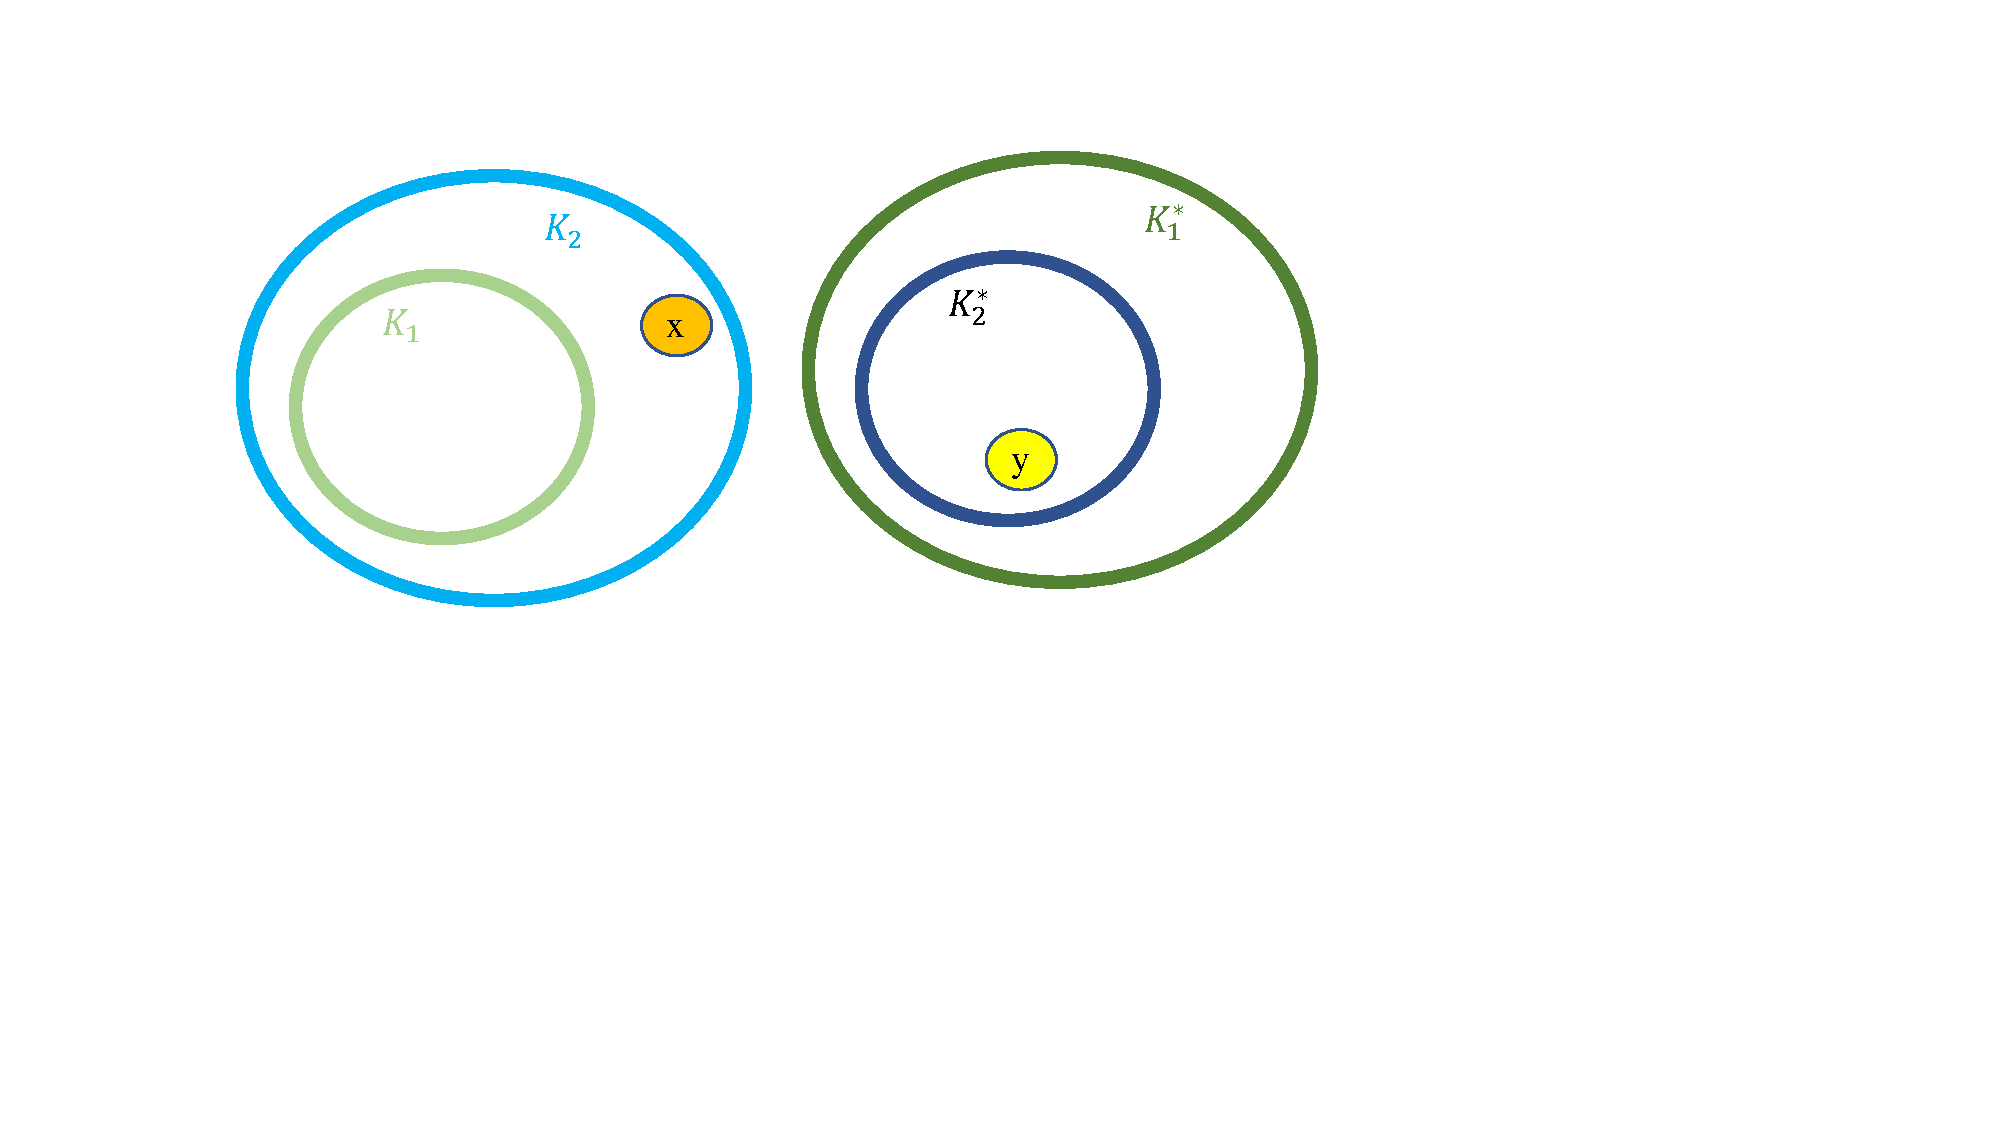
\includegraphics[width=0.65\textwidth]{fig/v.pdf}}
   \caption{Illustration to the argument made in 2.31(b).}
   \label{fig:v}
\end{figure}


\paragraph{Problem 2.32} The dual cone of $\left\lbrace Ax | x \succeq 0 \right\rbrace$ where $A \in \mathcal{R}^{m \times n}$ can be defined as $\left\lbrace x | A^{T}x \succeq 0 \right\rbrace$.
\bibliography{mybib}


\end{document}
